\documentclass{article} % Класс печатного документа

\usepackage{hyperref} % Для вставки гиперссылок
\usepackage{listings} % Для вставки кусков кода
\usepackage{graphicx} % Вставка изображений
\usepackage[utf8]{inputenc} % Кодировка исходного текста - utf8
\usepackage[english,russian]{babel} % Поддержка языка - русского с английским
\usepackage{indentfirst} % Отступ в первом абзаце

\title{Отчёт 1\protect\\Кластерный анализ} % Заголовок документа
\author{Свичкарев А.\,В.} % Автор документа
\date{\today} % Текущая дата

\begin{document} % Конец преамбулы, начало текста

\maketitle % Печатает заголовок, список авторов и дату

\section{Цель}
Изучить способы решения задач поиска кластеров в данных.

\section{Задание №1}
Написать программу формирования данных случайных кластеров и
их кластерного анализа по алгоритму <<associative clustering>> с пороговым значением 0.12.
Визуализировать в виде графика и сохранить файл изображения графика кластеров.

\clearpage

Реализация взята из Приложения, произведён рефакторинг и разобран алгоритм.
Выборки для разных алгоритмов были одинаков, чтобы можно было провести сравнение.

\noindent\makebox[\textwidth]{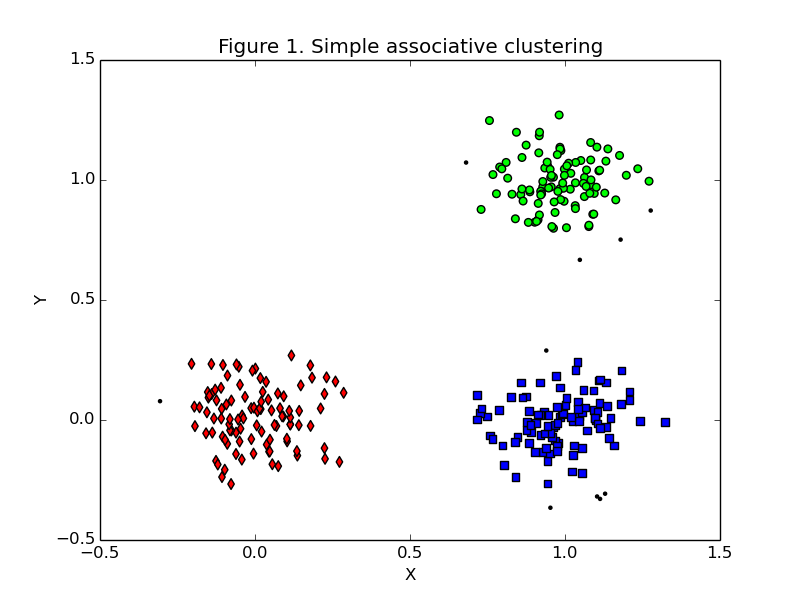
\includegraphics[width=0.7\paperwidth]{Figure_1}}

В разделе приложения представлено две разновидности алгоритма:
простой алгоритм кластеризации и вариант с очистрой от шума.

Для обоих вариантах вначале вычисляется матрица попарных расстояний в эвклидовой метрике между всеми вершинами.
Если расстояние меньше заданного порога, то вершины считаются соседними.
Основной шаг формирования кластеров заключается в слиянии всех вершин, являющихся соседями.
Слияние продолжается также по транзитивности,
т.е. если вершина А является соседней к B,
а B к C, то C считается соседом A и добавляется в кластер.
Кластер считается заполненным, когда кончаются соседи.
Благодаря транзитивности алгоритм работает быстро,
однако такая транзитивность не всегда может вести к хорошим результатам.

Второй вариант алгоритма аналогичен,
только к нему добавляются проверки числа соседей для вершин.
Если соседей вершины меньше порога, то она считается выбросом - шумом.

\clearpage

Выделенные кластера без шума:

\noindent\makebox[\textwidth]{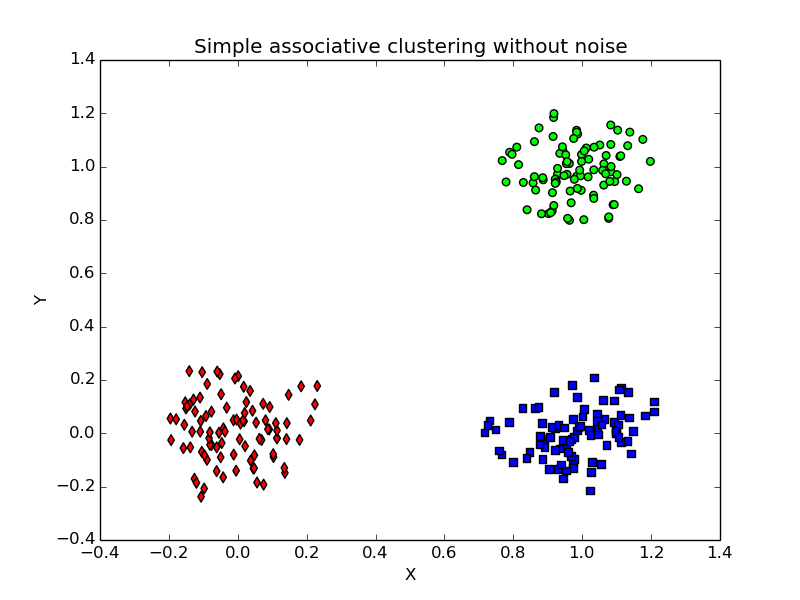
\includegraphics[width=0.7\paperwidth]{Figure_4}}

В секции Исходный код представлена реализация.

\section{Задание №2}
Для простых функций, имеющих реализацию в языке R была реализована функция вызова:
%\lstinputlisting[language=Python, firstline=5, lastline=8]{../code8.py}

С помощью функции вызова функции вычисления характеристик дескриптивной статистики реализуются в одну строчку:
%\lstinputlisting[language=Python, firstline=19, lastline=32]{../code8.py}

Для нахождения моды не получилось найти простого аналога в языке R, поэтому пришлось объявить и вызвать свою реализацию:
%\lstinputlisting[language=Python, firstline=35, lastline=44]{../code8.py}

В секции Исходный код представлены тесты и ожидаемые результаты на указанной в задание выборке.

\section{Задание №3}
Для аналога доверительного интервала в R не нашёл способа получить половину длины интервала, поэтому в Python взял правую границу и вычел среднее выборочное.

%\lstinputlisting[language=Python, firstline=47, lastline=50]{../code8.py}

В секции Исходный код представлен тест линейной регрессии с фиксированными значениями псевдо-генеротора чисел.

\section{Задание №4}
Выборки были сгенерированы внутри R, там же была вызвана функция lm, из вывода которой были получены коэффициенты.
\newpage
%\lstinputlisting[language=Python, firstline=53, lastline=62]{../code8.py}

\section{Задание №5}
Код R считывается из файла в Python и затем запускается:
%\lstinputlisting[language=Python, firstline=65, lastline=72]{../code8.py}
\newpage
Выборки были сгенерированы внутри R, там же была вызвана функция lm, построен график выборок и линейной регрессии и затем сохранён в виде png файла:

%\noindent\makebox[\textwidth]{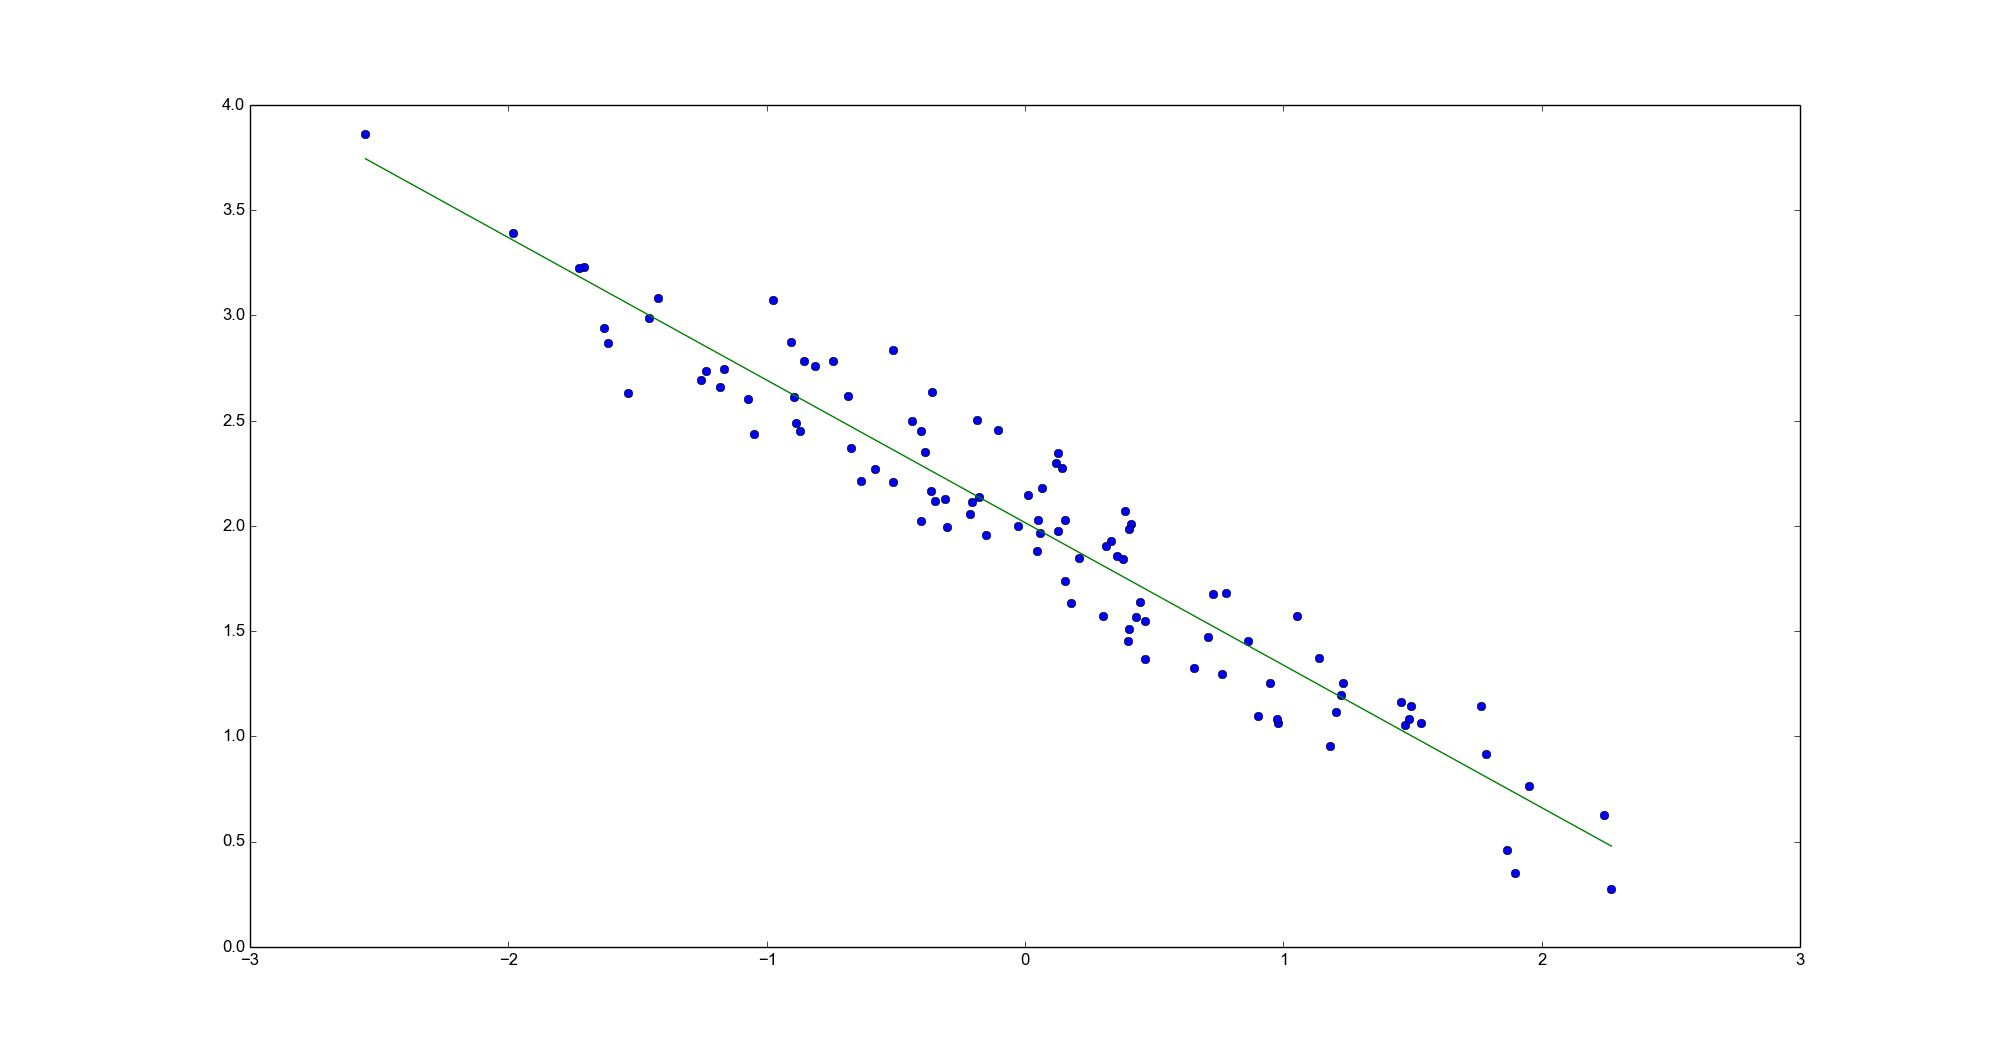
\includegraphics[width=0.7\paperwidth]{figure_1}}

\section{Пояснение}
Исходный код доступен по ссылке:

\href{https://github.com/SvichkarevAnatoly/Course-Python-Bioinformatics/tree/master/bioseq7}{https://github.com/SvichkarevAnatoly/Course-Python-Bioinformatics/tree/master/bioseq8}

\section{Исходный код}
Файл \verb$test_code8.py$:
%\lstinputlisting[language=Python]{../test_code8.py}

Файл \verb$r_lr_plot.R$:
%\lstinputlisting[language=Python]{../r_lr_plot.R}

\end{document} % Конец документа
